\documentclass[11pt,a4paper]{article}
\usepackage[utf8]{inputenc}
\usepackage[T1]{fontenc}
\usepackage{amsmath}
\usepackage{amssymb}
\usepackage{makeidx}
\usepackage{graphicx}
\usepackage[width=16.00cm, height=23.00cm]{geometry}
\usepackage{float}
\usepackage{indentfirst}
\setlength{\parindent}{4mm}
\setlength{\parskip}{1mm}

\usepackage{color}   %May be necessary if you want to color links
\usepackage{hyperref}
\hypersetup{
	colorlinks=true, %set true if you want colored links
	linktoc=all,     %set to all if you want both sections and subsections linked
	linkcolor=blue,  %choose some color if you want links to stand out
}

%------------------------------------
\usepackage{tikz}
\usepackage{pgfplots}
%\DeclareUnicodeCharacter{2212}{−}
\usepgfplotslibrary{groupplots,dateplot}
\usetikzlibrary{patterns,shapes.arrows}
%\pgfplotsset{compat=newest}
%------------------------------------------
\usepackage{listings}

\usepackage{xcolor}

\definecolor{codegreen}{rgb}{0,0.6,0}
\definecolor{codegray}{rgb}{0.5,0.5,0.5}
\definecolor{codepurple}{rgb}{0.58,0,0.82}
\definecolor{backcolour}{rgb}{0.95,0.95,0.92}

\lstdefinestyle{mystyle}{
	backgroundcolor=\color{backcolour},   
	commentstyle=\color{codegreen},
	keywordstyle=\color{magenta},
	numberstyle=\tiny\color{codegray},
	stringstyle=\color{codepurple},
	basicstyle=\ttfamily\footnotesize,
	breakatwhitespace=false,         
	breaklines=true,                 
	captionpos=b,                    
	keepspaces=true,                 
	numbers=left,                    
	numbersep=5pt,                  
	showspaces=false,                
	showstringspaces=false,
	showtabs=true,                  
	tabsize=2,
}

\lstset{style=mystyle}

\usepackage{verbatim}
\usepackage{fancyvrb}
%----------------------------------------------------------------------

\author{Pritish Karmakar}

	

\begin{document}
	\begin{titlepage}
		\centering
		
\includegraphics[width=2.5cm]{iiserk.png}
		
		\vspace{4cm}
		{\Huge\bfseries Summer Project 2023}
		
		\vspace{3cm}
		{\LARGE Pritish Karmakar\\}
		\vspace{0.3cm}
		{21MS179}
		\vfill
		
		
		\clearpage
		\tableofcontents
		\clearpage
		\listoffigures
		\listoftables
	\end{titlepage}
	
\section{Gaussian curve and its fourier transform}
%Figure \ref{fig:gaussian} shows a gaussian curve.

%\noindent \dotfill \textbf{Code Block} \noindent\dotfill
%\verbatiminput{gaussian.py}

%\dotfill

\subsection{Standard normal}
\lstinputlisting[language=Python, firstline=1, lastline=14]{gaussian.py}
\begin{figure}[ht]
	\centering
	\scalebox{1}{% This file was created with tikzplotlib v0.10.1.
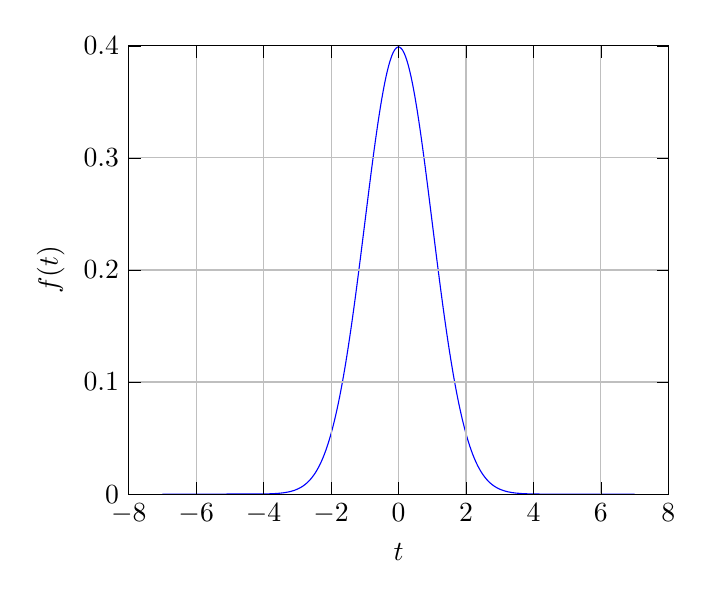
\begin{tikzpicture}

\begin{axis}[
axis on top,
tick pos=both,
xlabel=\textcolor{black}{\(\displaystyle t\)},
xmajorgrids,
xmin=-8, xmax=8,
xtick style={color=black},
ylabel=\textcolor{black}{\(\displaystyle f(t)\)},
ymajorgrids,
ymin=0, ymax=0.4,
ytick style={color=black}
]
\addplot [blue]
table {%
-7 0
-4.05705690383911 0.000106334686279297
-3.76276278495789 0.000336050987243652
-3.56656646728516 0.00068974494934082
-3.41241240501404 0.00118124485015869
-3.28628635406494 0.00180208683013916
-3.17417407035828 0.00258862972259521
-3.0760760307312 0.0035172700881958
-2.99199199676514 0.00453948974609375
-2.92192196846008 0.00558459758758545
-2.85185194015503 0.00683653354644775
-2.7817816734314 0.00832831859588623
-2.72572565078735 0.00971841812133789
-2.66966962814331 0.0113050937652588
-2.61361360549927 0.0131094455718994
-2.55755758285522 0.0151540040969849
-2.50150156021118 0.0174626111984253
-2.45945954322815 0.0193819999694824
-2.41741752624512 0.0214744806289673
-2.37537527084351 0.0237506628036499
-2.33333325386047 0.0262218713760376
-2.29129123687744 0.028899073600769
-2.24924921989441 0.0317933559417725
-2.20720720291138 0.0349156856536865
-2.16516518592834 0.0382769107818604
-2.12312316894531 0.041887640953064
-2.08108115196228 0.0457580089569092
-2.03903913497925 0.0498977899551392
-1.99699699878693 0.0543159246444702
-1.95495498180389 0.05902099609375
-1.91291296482086 0.0640201568603516
-1.87087082862854 0.0693203210830688
-1.82882881164551 0.0749266147613525
-1.78678679466248 0.0808433294296265
-1.74474477767944 0.0870732069015503
-1.70270276069641 0.0936175584793091
-1.66066062450409 0.100476145744324
-1.61861860752106 0.107646584510803
-1.57657659053802 0.115125179290771
-1.53453457355499 0.122905850410461
-1.49249243736267 0.130980730056763
-1.45045042037964 0.139339447021484
-1.40840840339661 0.147969961166382
-1.36636638641357 0.15685760974884
-1.32432436943054 0.165985345840454
-1.28228223323822 0.175333976745605
-1.24024021625519 0.184882164001465
-1.18418419361115 0.197881937026978
-1.1281281709671 0.21113133430481
-1.05805802345276 0.227937936782837
-0.861861944198608 0.275176763534546
-0.805805802345276 0.288344264030457
-0.763763785362244 0.298016548156738
-0.721721649169922 0.307469367980957
-0.67967963218689 0.316661834716797
-0.637637615203857 0.325553178787231
-0.609609603881836 0.33129358291626
-0.581581592559814 0.336870431900024
-0.553553581237793 0.342272043228149
-0.525525569915771 0.347487330436707
-0.49749755859375 0.352504968643188
-0.469469428062439 0.357314348220825
-0.441441416740417 0.361904859542847
-0.413413405418396 0.36626660823822
-0.385385394096375 0.370389699935913
-0.357357382774353 0.374265193939209
-0.329329371452332 0.377884149551392
-0.301301240921021 0.381238698959351
-0.273273229598999 0.384320735931396
-0.245245218276978 0.387123584747314
-0.217217206954956 0.389640688896179
-0.189189195632935 0.391866207122803
-0.161161184310913 0.393794894218445
-0.133133172988892 0.395422458648682
-0.10510516166687 0.396744728088379
-0.0770770311355591 0.397758960723877
-0.0490490198135376 0.398462653160095
-0.0210210084915161 0.39885413646698
0.00700700283050537 0.398932456970215
0.0350350141525269 0.39869749546051
0.0630630254745483 0.398149728775024
0.0910910367965698 0.397290587425232
0.119119167327881 0.396121978759766
0.147147178649902 0.394646525382996
0.175175189971924 0.392867922782898
0.203203201293945 0.390790224075317
0.231231212615967 0.388418316841125
0.259259223937988 0.385757565498352
0.28728723526001 0.382814168930054
0.315315246582031 0.379595041275024
0.343343377113342 0.376107215881348
0.371371388435364 0.372359037399292
0.399399399757385 0.368358612060547
0.427427411079407 0.364114999771118
0.455455422401428 0.35963761806488
0.483483552932739 0.354936361312866
0.511511564254761 0.350021600723267
0.539539575576782 0.344903707504272
0.567567586898804 0.339593887329102
0.595595598220825 0.334103107452393
0.623623609542847 0.328443050384521
0.665665626525879 0.319661140441895
0.707707643508911 0.310564517974854
0.749749660491943 0.301193952560425
0.791791796684265 0.291590213775635
0.847847819328308 0.278493165969849
0.903903961181641 0.26514995098114
0.987987995147705 0.244877099990845
1.10010015964508 0.217828154563904
1.17017018795013 0.201173543930054
1.22622621059418 0.188105225563049
1.26826822757721 0.178495645523071
1.31031036376953 0.16907799243927
1.35235238075256 0.159874320030212
1.3943943977356 0.150904774665833
1.43643641471863 0.142186880111694
1.47847843170166 0.13373601436615
1.52052056789398 0.12556529045105
1.56256258487701 0.117685556411743
1.60460460186005 0.110105514526367
1.64664661884308 0.102831721305847
1.68868863582611 0.0958689451217651
1.73073077201843 0.0892196893692017
1.77277278900146 0.0828850269317627
1.8148148059845 0.0768642425537109
1.85685682296753 0.0711548328399658
1.89889883995056 0.0657532215118408
1.94094097614288 0.0606542825698853
1.98298299312592 0.0558520555496216
2.02502512931824 0.0513391494750977
2.06706714630127 0.0471075773239136
2.1091091632843 0.043148398399353
2.15115118026733 0.0394521951675415
2.19319319725037 0.0360089540481567
2.2352352142334 0.0328081846237183
2.27727723121643 0.0298391580581665
2.31931924819946 0.0270907878875732
2.3613612651825 0.0245522260665894
2.40340352058411 0.0222122669219971
2.44544553756714 0.0200597047805786
2.48748755455017 0.0180838108062744
2.54354357719421 0.0157054662704468
2.59959959983826 0.0135971307754517
2.6556556224823 0.0117348432540894
2.71171164512634 0.0100958347320557
2.76776766777039 0.00865852832794189
2.83783793449402 0.00711464881896973
2.90790796279907 0.00581741333007812
2.97797799110413 0.00473332405090332
3.06206202507019 0.00367188453674316
3.14614605903625 0.00282835960388184
3.24424433708191 0.00206732749938965
3.35635638237 0.00142800807952881
3.48248243331909 0.00092768669128418
3.63663673400879 0.000535964965820312
3.84684681892395 0.000244021415710449
4.15515518188477 7.10487365722656e-05
4.7717719078064 4.52995300292969e-06
7 0
};
\end{axis}

\end{tikzpicture}
}
	\caption{Standard Normal curve}
	\label{fig:gaussian}
\end{figure}


\subsection{Fourier transform of Standard normal}
If $f(t)=\int_{-\infty}^{\infty}g(\omega)e^{i\omega t} d\omega$, then fourier transform of that is $g(\omega)=\frac{1}{2\pi}\int_{-\infty}^{\infty}f(t)e^{-i\omega t} dt$. Here, $f(x)=\frac{1}{\sqrt{2\pi}}e^{-x^2 /2}$\\

\begin{align*}
	g(\omega)&=\frac{1}{2\pi}\int_{-\infty}^{\infty}f(t)e^{-i\omega t} dt\\
	&=\frac{1}{2\pi}\int_{-\infty}^{\infty}f(t)\cos(\omega t) dt - i \frac{1}{2\pi}\int_{-\infty}^{\infty}f(t)\sin(\omega t) dt
\end{align*}


\lstinputlisting[language=Python, firstline=1, lastline=21]{fft_gaussian.py}


\begin{figure}[ht]
	\centering
	\scalebox{1}{% This file was created with tikzplotlib v0.10.1.
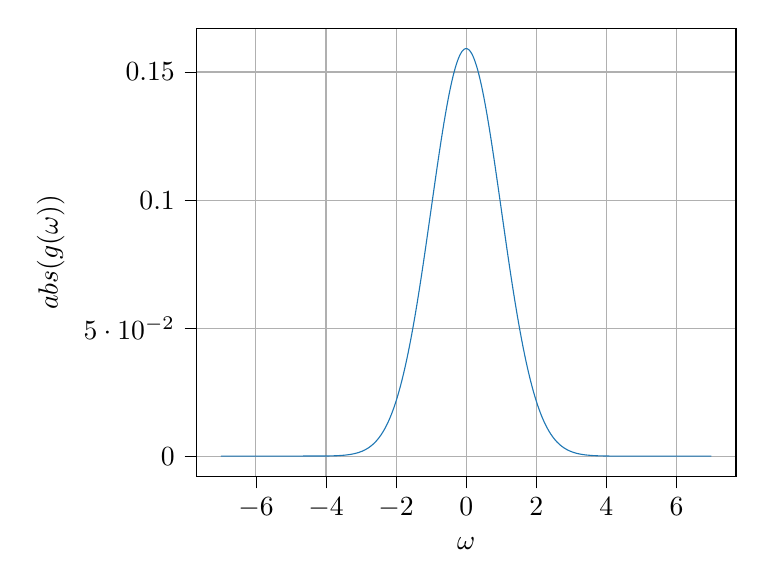
\begin{tikzpicture}

\definecolor{darkgray176}{RGB}{176,176,176}
\definecolor{steelblue31119180}{RGB}{31,119,180}

\begin{axis}[
tick align=outside,
tick pos=left,
x grid style={darkgray176},
xlabel={\(\displaystyle \omega\)},
xmajorgrids,
xmin=-7.7, xmax=7.7,
xtick style={color=black},
y grid style={darkgray176},
ylabel={\(\displaystyle abs(g(\omega))\)},
ymajorgrids,
ymin=-0.00795755179784204, ymax=0.167108587834931,
ytick style={color=black}
]
\addplot [steelblue31119180]
table {%
-7 0
-3.97297286987305 5.94854354858398e-05
-3.66466474533081 0.000192999839782715
-3.46846842765808 0.000388622283935547
-3.31431436538696 0.000655412673950195
-3.18818807601929 0.000987648963928223
-3.0760760307312 0.00140321254730225
-2.97797799110413 0.00188839435577393
-2.89389395713806 0.00241708755493164
-2.809809923172 0.00307214260101318
-2.73973965644836 0.003731369972229
-2.66966962814331 0.00451004505157471
-2.59959959983826 0.00542449951171875
-2.54354357719421 0.00626564025878906
-2.48748755455017 0.00721442699432373
-2.43143153190613 0.00828087329864502
-2.37537527084351 0.00947511196136475
-2.31931924819946 0.0108076333999634
-2.26326322555542 0.0122889280319214
-2.22122120857239 0.0135037899017334
-2.17917919158936 0.0148124694824219
-2.13713717460632 0.0162192583084106
-2.09509515762329 0.017728328704834
-2.05305314064026 0.0193436145782471
-2.01101112365723 0.021068811416626
-1.9689689874649 0.0229073762893677
-1.92692697048187 0.0248622894287109
-1.88488483428955 0.0269365310668945
-1.84284281730652 0.0291321277618408
-1.80080080032349 0.0314512252807617
-1.75875878334045 0.0338947772979736
-1.71671676635742 0.0364638566970825
-1.6746746301651 0.0391582250595093
-1.63263261318207 0.0419775247573853
-1.59059059619904 0.0449202060699463
-1.548548579216 0.0479844808578491
-1.50650656223297 0.0511671304702759
-1.46446442604065 0.05446457862854
-1.42242240905762 0.0578720569610596
-1.38038039207458 0.0613842010498047
-1.33833837509155 0.0649945735931396
-1.28228223323822 0.0699481964111328
-1.22622621059418 0.0750430822372437
-1.17017018795013 0.0802565813064575
-1.10010015964508 0.0869008302688599
-0.987987995147705 0.0976918935775757
-0.875875949859619 0.108451008796692
-0.819819808006287 0.11372983455658
-0.763763785362244 0.118891477584839
-0.721721649169922 0.122662544250488
-0.67967963218689 0.126329779624939
-0.637637615203857 0.129876971244812
-0.595595598220825 0.133287906646729
-0.553553581237793 0.136546850204468
-0.511511564254761 0.139638423919678
-0.483483552932739 0.141599178314209
-0.455455422401428 0.143474698066711
-0.427427411079407 0.145260810852051
-0.399399399757385 0.146953821182251
-0.371371388435364 0.148549795150757
-0.343343377113342 0.150045156478882
-0.315315246582031 0.151436448097229
-0.28728723526001 0.152720808982849
-0.259259223937988 0.153895020484924
-0.231231212615967 0.154956459999084
-0.203203201293945 0.155902743339539
-0.175175189971924 0.156731605529785
-0.147147178649902 0.157441139221191
-0.119119167327881 0.158029794692993
-0.0910910367965698 0.158496022224426
-0.0630630254745483 0.158838748931885
-0.0350350141525269 0.159057259559631
-0.00700700283050537 0.159151077270508
0.0210210084915161 0.159119844436646
0.0490490198135376 0.158963561058044
0.0770770311355591 0.158682823181152
0.10510516166687 0.158278226852417
0.133133172988892 0.157750725746155
0.161161184310913 0.157101392745972
0.189189195632935 0.156332015991211
0.217217206954956 0.155444145202637
0.245245218276978 0.154439926147461
0.273273229598999 0.153321862220764
0.301301240921021 0.152092218399048
0.329329371452332 0.150753974914551
0.357357382774353 0.149310231208801
0.385385394096375 0.147764086723328
0.413413405418396 0.146119236946106
0.441441416740417 0.144379138946533
0.469469428062439 0.142547845840454
0.49749755859375 0.140629172325134
0.539539575576782 0.137596607208252
0.581581592559814 0.134391784667969
0.623623609542847 0.131029844284058
0.665665626525879 0.12752628326416
0.707707643508911 0.123897314071655
0.749749660491943 0.120159029960632
0.805805802345276 0.11503267288208
0.861861944198608 0.109779715538025
0.931931972503662 0.103092789649963
1.15615618228912 0.0815755128860474
1.21221220493317 0.0763363838195801
1.26826822757721 0.0712094306945801
1.32432436943054 0.0662186145782471
1.36636638641357 0.0625771284103394
1.40840840339661 0.0590314865112305
1.45045042037964 0.0555884838104248
1.49249243736267 0.0522537231445312
1.53453457355499 0.0490323305130005
1.57657659053802 0.0459282398223877
1.61861860752106 0.0429447889328003
1.66066062450409 0.0400841236114502
1.70270276069641 0.0373480319976807
1.74474477767944 0.034737229347229
1.78678679466248 0.0322518348693848
1.82882881164551 0.0298913717269897
1.87087082862854 0.027654767036438
1.91291296482086 0.0255403518676758
1.95495498180389 0.0235459804534912
1.99699699878693 0.0216689109802246
2.03903913497925 0.0199062824249268
2.08108115196228 0.0182547569274902
2.12312316894531 0.0167107582092285
2.16516518592834 0.0152702331542969
2.20720720291138 0.0139293670654297
2.24924921989441 0.0126837491989136
2.30530524253845 0.011163592338562
2.3613612651825 0.00979495048522949
2.41741752624512 0.00856709480285645
2.47347354888916 0.00746965408325195
2.5295295715332 0.0064922571182251
2.58558559417725 0.00562512874603271
2.6556556224823 0.00468158721923828
2.72572565078735 0.00387704372406006
2.79579567909241 0.00319516658782959
2.87987995147705 0.00251686573028564
2.96396398544312 0.0019686222076416
3.06206202507019 0.00146484375
3.16016006469727 0.00107955932617188
3.27227234840393 0.000752806663513184
3.41241240501404 0.000471234321594238
3.58058047294617 0.000261783599853516
3.80480480194092 0.000114321708679199
4.14114093780518 3.00407409667969e-05
4.86986970901489 1.07288360595703e-06
7 0
};
\end{axis}

\end{tikzpicture}
}
	\caption{Fourier transform of Standard Normal}
	\label{fig:fft_gaussian}
\end{figure}
\clearpage

\section{Gaussian beam}

\subsection{Intensity profile}

\lstinputlisting[language=Python, firstline=4, lastline=19]{intensity_gaussian.py}

\begin{figure}[htbp]
	\centering
	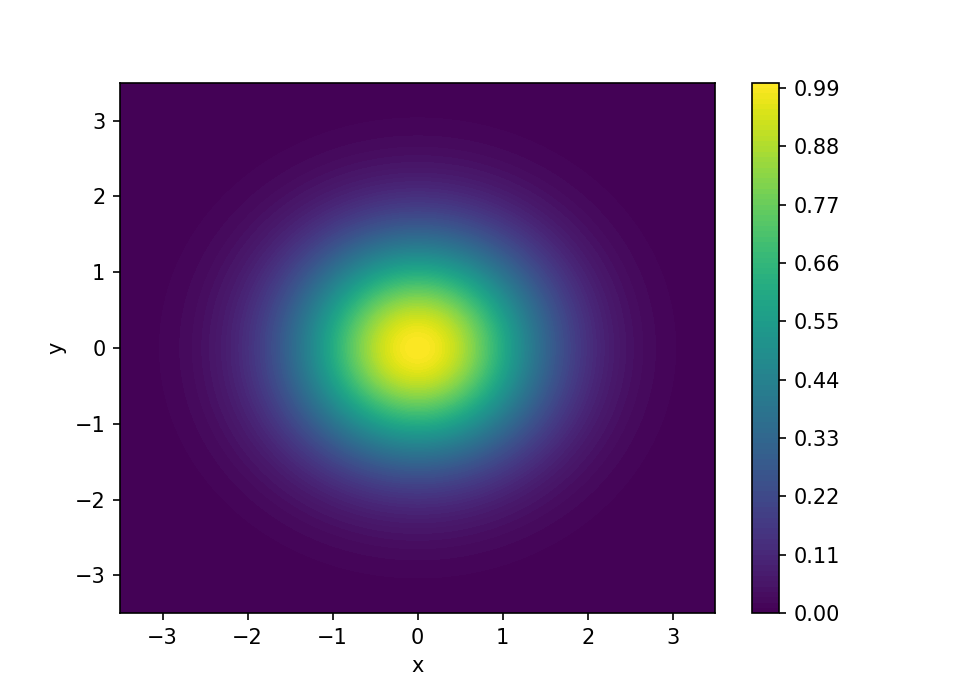
\includegraphics[width=9cm]{intensity.png}
	\caption{Intensity variation in a cross section ($z=0,z_0=1$)}
	\label{fig:intensity}
\end{figure}



\lstinputlisting[language=Python, firstline=4, lastline=20]{intensity_var.py}

\begin{figure}[H]
	\centering
	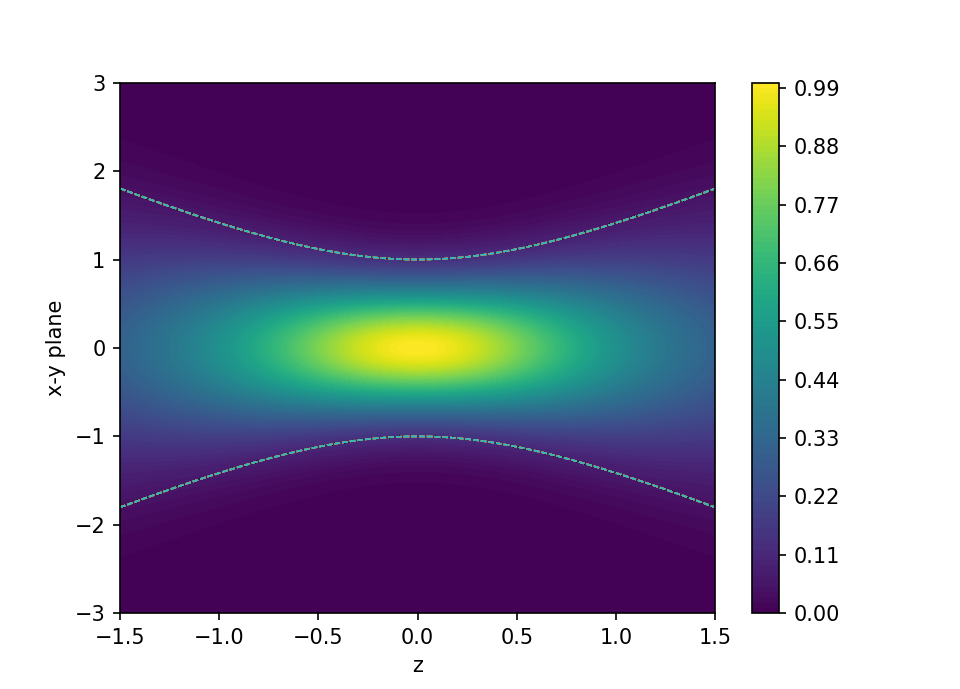
\includegraphics[width=9cm]{intensity_var.png}
	\caption{Intensity variation along z ($z_0=1$)}
	\label{fig:intensity_var}
\end{figure}




\end{document}